% ============================================================
%  COMPTE RENDU — TD N°05 — Arbres de Décision & KNN
%  Chabbaki Ayman — G1 — MDSBDIA26
%  Master Intelligence Artificielle — Semestre 2024-2025
% ============================================================

\documentclass[12pt,a4paper]{article}

% ─── Encodage & Langue ───────────────────────────────────────
\usepackage[utf8]{inputenc}
\usepackage[T1]{fontenc}
\usepackage[french]{babel}

% ─── Mise en page ────────────────────────────────────────────
\usepackage[top=2.5cm,bottom=2.5cm,left=2.5cm,right=2.5cm,
            headheight=15pt]{geometry}
\usepackage{fancyhdr}
\usepackage{titlesec}
\usepackage{microtype}
\usepackage{parskip}

% ─── Mathématiques ───────────────────────────────────────────
\usepackage{amsmath,amssymb,amsfonts}

% ─── Figures & Tables ────────────────────────────────────────
\usepackage{graphicx}
\usepackage{float}
\usepackage{subcaption}
\usepackage{booktabs}
\usepackage{array}
\usepackage{xcolor}
\usepackage{colortbl}
\usepackage{multirow}
\usepackage{tabularx}
\usepackage{caption}

% ─── Code ────────────────────────────────────────────────────
\usepackage{listings}

% ─── Boîtes colorées ─────────────────────────────────────────
\usepackage{tcolorbox}
\tcbuselibrary{skins,breakable}

% ─── Divers ──────────────────────────────────────────────────
\usepackage{hyperref}
\usepackage{enumitem}
\usepackage{setspace}
\usepackage{lmodern}

% ─── Palette de couleurs ─────────────────────────────────────
\definecolor{darkblue}{RGB}{26,37,80}
\definecolor{teal}{RGB}{26,122,110}
\definecolor{crimson}{RGB}{156,61,56}
\definecolor{amber}{RGB}{176,125,58}
\definecolor{purple}{RGB}{91,61,143}
\definecolor{lightblue}{RGB}{232,240,255}
\definecolor{lightteal}{RGB}{232,247,244}
\definecolor{codebg}{RGB}{248,248,248}
\definecolor{rowalt}{RGB}{241,245,255}

% ─── Style des sections ──────────────────────────────────────
\titleformat{\section}[block]
  {\large\bfseries\color{darkblue}}
  {\thesection}{1em}{}
  [\vspace{-4pt}\color{darkblue}\rule{\linewidth}{0.6pt}\vspace{2pt}]

\titleformat{\subsection}[block]
  {\normalsize\bfseries\color{teal}}
  {\thesubsection}{1em}{}

\titleformat{\subsubsection}[block]
  {\normalsize\bfseries\color{amber}}
  {\thesubsubsection}{0.8em}{}

% ─── Style Python ────────────────────────────────────────────
\lstdefinestyle{python}{
  language=Python,
  basicstyle=\ttfamily\scriptsize,
  keywordstyle=\color{darkblue}\bfseries,
  stringstyle=\color{crimson},
  commentstyle=\color{teal!80!black}\itshape,
  numberstyle=\tiny\color{gray},
  numbers=left,
  stepnumber=1,
  backgroundcolor=\color{codebg},
  frame=single,
  framerule=0.4pt,
  rulecolor=\color{darkblue!25},
  breaklines=true,
  showstringspaces=false,
  tabsize=4,
  xleftmargin=18pt,
  xrightmargin=5pt,
  aboveskip=6pt,
  belowskip=4pt,
}
\lstset{style=python}

% ─── Environnements tcolorbox ─────────────────────────────────
\newtcolorbox{reponsebox}[1][]{
  enhanced, breakable,
  title={\small Analyse — #1},
  fonttitle=\bfseries\small,
  colback=lightteal,
  colframe=teal,
  colbacktitle=teal,
  coltitle=white,
  boxrule=0.5pt,
  arc=4pt,
  top=4pt, bottom=4pt, left=6pt, right=6pt,
}

\newtcolorbox{resultbox}[1][Résultats expérimentaux]{
  enhanced, breakable,
  title={\small #1},
  fonttitle=\bfseries\small,
  colback=lightblue,
  colframe=darkblue,
  colbacktitle=darkblue,
  coltitle=white,
  boxrule=0.5pt,
  arc=4pt,
}

\newtcolorbox{observbox}[1][Observation]{
  enhanced, breakable,
  title={\small #1},
  fonttitle=\bfseries\small,
  colback=amber!10!white,
  colframe=amber,
  colbacktitle=amber,
  coltitle=white,
  boxrule=0.5pt,
  arc=4pt,
}

% ─── En-tête / pied de page ──────────────────────────────────
\pagestyle{fancy}
\fancyhf{}
\fancyhead[L]{\small\color{darkblue!70}Master IA — TD\,5 : Arbres de Décision \& KNN}
\fancyhead[R]{\small\color{darkblue!70}Chabbaki Ayman — Groupe G1}
\fancyfoot[C]{\small\thepage}
\renewcommand{\headrulewidth}{0.4pt}
\renewcommand{\footrulewidth}{0.2pt}

% ─── Hyperref ────────────────────────────────────────────────
\hypersetup{
  colorlinks=true,
  linkcolor=darkblue,
  urlcolor=crimson,
  pdftitle={Compte Rendu TD5 — Arbres et KNN},
  pdfauthor={Chabbaki Ayman},
}

% ─── Commandes utilitaires ───────────────────────────────────
\newcommand{\feature}[1]{\texttt{\small #1}}
\newcommand{\algo}[1]{\textit{#1}}
\newcommand{\score}[1]{\textbf{#1}}

% ═════════════════════════════════════════════════════════════
\begin{document}

% ─── PAGE DE TITRE ───────────────────────────────────────────
\begin{titlepage}
  \thispagestyle{empty}

  % Bande supérieure
  \noindent
  \colorbox{darkblue}{\parbox{\linewidth}{%
    \vspace{8pt}
    \centering
    \color{white}\large\textbf{Université — Master Intelligence Artificielle}\\[4pt]
    \color{white}\normalsize Module : Machine Learning — Semestre 2024–2025
    \vspace{8pt}
  }}

  \vspace{2.5cm}

  % Titre principal
  \begin{center}
    {\color{darkblue}\rule{0.85\linewidth}{1.5pt}}\\[18pt]
    {\Huge\bfseries\color{darkblue} Compte Rendu}\\[10pt]
    {\huge\bfseries\color{teal} TD N°\,05}\\[14pt]
    {\LARGE\bfseries Arbres de Décision}\\[6pt]
    {\LARGE\bfseries\color{crimson} \&\ K-Nearest Neighbors (KNN)}\\[18pt]
    {\color{darkblue}\rule{0.85\linewidth}{1.5pt}}
  \end{center}

  \vspace{2.5cm}

  % Informations étudiant
  \begin{center}
    \begin{tabular}{rl}
      \toprule
      \textbf{Étudiant}     & Chabbaki Ayman \\[4pt]
      \textbf{Groupe}       & G1 \\[4pt]
      \textbf{Promotion}    & MDSBDIA26 \\[4pt]
      \textbf{Dataset}      & BankChurners \\[4pt]
      \textbf{Outils}       & Python 3.10, scikit-learn, NumPy, Matplotlib \\[4pt]
      \bottomrule
    \end{tabular}
  \end{center}

  \vspace{2cm}

  % Professeur
  \begin{center}
    {\large Encadrant : \textbf{Pr.\ BEN LAHMAR EL Habib}}
  \end{center}

  \vfill

  % Bande inférieure
  \noindent
  \colorbox{teal}{\parbox{\linewidth}{%
    \vspace{6pt}
    \centering
    \color{white}\small
    Master Intelligence Artificielle — Arbres de Décision \& KNN
    \vspace{6pt}
  }}
\end{titlepage}

\newpage
\tableofcontents
\newpage

% ─────────────────────────────────────────────────────────────
\section{Introduction et Rappels Théoriques}
% ─────────────────────────────────────────────────────────────

Ce TD met en parallèle deux algorithmes aux philosophies opposées : l'\textbf{Arbre de Décision}
— interprétable, basé sur des règles SI/ALORS — et le \textbf{KNN} — non-paramétrique,
basé sur la distance. Les deux ont des forces complémentaires selon le contexte.

\subsection{Arbre de Décision — Construction et Critères de Split}

Le principe de l'arbre de décision est de partitionner récursivement l'espace des features
par des questions binaires ($x_i \leq \text{seuil}$\,?). Les algorithmes principaux sont :
ID3 (entropie, données discrètes), C4.5 (entropie, continu + manquants), CART (Gini, utilisé
par \texttt{sklearn}).

\textbf{Critères d'impureté :}
\begin{align}
  \text{Entropie de Shannon :} &\quad H(S) = -\sum_{i} p_i \log_2(p_i)
    \quad \text{(Nœud pur : }H=0\text{; Aléatoire : }H=1\text{)}\\[4pt]
  \text{Impureté de Gini :} &\quad G(S) = 1 - \sum_{i} p_i^2
    \quad \text{(Nœud pur : }G=0\text{; Maximum : }G=0{,}5\text{)}\\[4pt]
  \text{Gain d'information :} &\quad IG(S,A) = H(S) - \sum_{v}
    \frac{|S_v|}{|S|} H(S_v)
\end{align}

\subsection{K-Nearest Neighbors (KNN) — Algorithme et Propriétés}

KNN est un \emph{lazy learner} : aucun entraînement proprement dit — tout le calcul se fait à la prédiction.
Un nouveau point $\mathbf{x}$ est classifié par vote majoritaire de ses $K$ plus proches voisins selon la
distance euclidienne :
\begin{equation}
  d(\mathbf{x},\mathbf{y}) = \sqrt{\sum_{j=1}^{d}(x_j - y_j)^2}
\end{equation}

\begin{observbox}[Sensibilité à l'échelle]
La distance euclidienne est sensible aux différences d'échelle des features. Sans normalisation,
une feature à grande variance (ex.\ \feature{Credit\_Limit} avec $\sigma^2 \approx 81{,}6\times10^6$)
écrase totalement les autres dans le calcul de distance. La normalisation est donc \textbf{obligatoire}
pour KNN, mais inutile pour l'Arbre de Décision.
\end{observbox}

\subsection{Tableau comparatif théorique}

\begin{table}[H]
\centering
\caption{Comparaison théorique : Arbre de Décision vs KNN}
\begin{tabularx}{\linewidth}{lXX}
\toprule
\textbf{Critère} & \textbf{Arbre de Décision} & \textbf{KNN} \\
\midrule
Complexité entraînement & $O(n \cdot d \cdot \log n)$ & Aucune — lazy learner \\
\rowcolor{rowalt}
Complexité prédiction & $O(\text{profondeur}) \approx O(\log n)$ & $O(n \cdot d)$ — coûteux \\
Normalisation & Non requise & \textbf{Obligatoire} \\
\rowcolor{rowalt}
Interprétabilité & Très élevée — règles lisibles & Nulle — boîte noire \\
Hyperparamètre clé & \texttt{max\_depth}, \texttt{min\_samples\_leaf} & $K$ (nombre de voisins) \\
\rowcolor{rowalt}
Haute dimension & Se dégrade (overfitting) & Malédiction dimensionnalité \\
\bottomrule
\end{tabularx}
\end{table}

\subsection{Préparation de l'environnement et du dataset}

Le dataset \textbf{BankChurners} est encodé et partitionné avec les paramètres suivants :

\begin{resultbox}[Partition train/test — BankChurners]
\begin{itemize}[noitemsep]
  \item \textbf{Ensemble d'entraînement} : 8\,101 exemples $\times$ 19 features
  \item \textbf{Ensemble de test} : 2\,026 exemples $\times$ 19 features
  \item \textbf{Taux de churn (train)} : 1\,302 / 8\,101 $\approx$ \textbf{16,07\,\%}
    (distribution déséquilibrée : 83,93\,\% \emph{Existing} vs 16,07\,\% \emph{Attrited})
  \item \textbf{Stratégie} : stratification par classe, \texttt{random\_state=42}
\end{itemize}
\end{resultbox}

% ─────────────────────────────────────────────────────────────
\section{Partie 1 — Calculs Manuels : Entropie, Gini et Gain d'Information}
% ─────────────────────────────────────────────────────────────

\subsection{Q\,1.1 — Calcul manuel d'entropie et d'impureté de Gini}

\subsubsection{Implémentation Python}

\begin{lstlisting}[caption={Fonctions de calcul d'entropie et de Gini}]
def entropie(classes):
    total = sum(classes)
    if total == 0: return 0
    H = 0
    for n in classes:
        if n > 0:
            p = n / total
            H -= p * np.log2(p)
    return H

def gini(classes):
    total = sum(classes)
    if total == 0: return 0
    return 1 - sum((n/total)**2 for n in classes)
\end{lstlisting}

\subsubsection{Résultats obtenus}

\begin{table}[H]
\centering
\caption{Entropie et Gini pour cinq nœuds représentatifs}
\begin{tabular}{lrrcc}
\toprule
\textbf{Nœud} & \textbf{Classe 0} & \textbf{Classe 1} & \textbf{Entropie (bits)} & \textbf{Gini} \\
\midrule
A — Pur                 & 10  & 0   & \score{0.0000} & \score{0.0000} \\
\rowcolor{rowalt}
B — Équilibré           & 5   & 5   & \score{1.0000} & \score{0.5000} \\
C — Réel (83,9/16,1)    & 839 & 161 & \score{0.6367} & \score{0.2702} \\
\rowcolor{rowalt}
D — Gauche              & 600 & 40  & \score{0.3373} & \score{0.1172} \\
D — Droite              & 239 & 121 & \score{0.9210} & \score{0.4463} \\
\bottomrule
\end{tabular}
\end{table}

\subsubsection{Analyse}

\begin{reponsebox}[Q1 — Nœud pur A]
Pour le nœud A ($p_0=1,\;p_1=0$), les deux mesures valent \textbf{0}.
Démonstration : $H = -(1\cdot\log_2 1 + 0) = 0$ et $G = 1 - 1^2 = 0$.
Un nœud pur est l'objectif de l'arbre : il prédit avec une certitude de 100\,\% sans ambiguïté.
\end{reponsebox}

\begin{reponsebox}[Q2 — Nœud équilibré B]
Pour une distribution 50/50, l'incertitude est maximale :
\[
  H = -(0{,}5\log_2 0{,}5 + 0{,}5\log_2 0{,}5) = \mathbf{1{,}0} \text{ bit}
  \qquad
  G = 1 - (0{,}5^2 + 0{,}5^2) = \mathbf{0{,}5}
\]
Ces valeurs correspondent exactement aux maxima théoriques pour une classification binaire.
\end{reponsebox}

\begin{reponsebox}[Q3 — Entropie vs Gini sur le nœud C]
Pour la distribution réelle (83,9\,\% / 16,1\,\%) :
l'entropie $H = 0{,}6367 > G = 0{,}2702$ car la fonction logarithmique est plus sensible
aux déséquilibres de classes. En pratique, les deux critères produisent des arbres très similaires.
\texttt{sklearn} utilise Gini par défaut (plus rapide : pas de calcul logarithmique).
\end{reponsebox}

\subsection{Q\,1.2 — Gain d'information — Choisir le meilleur attribut de split}

\subsubsection{Résultats}

\begin{table}[H]
\centering
\caption{Comparaison du gain d'information pour deux features}
\begin{tabular}{lcc}
\toprule
\textbf{Feature} & \textbf{Seuil optimal} & \textbf{IG maximal} \\
\midrule
\feature{Total\_Trans\_Ct}         & $\leq 60{,}0$ & \score{0.12213} \\
\rowcolor{rowalt}
\feature{Months\_Inactive\_12\_mon} & $\leq 1{,}0$  & \score{0.02497} \\
\bottomrule
\multicolumn{3}{l}{\small $\Rightarrow$ \textbf{Meilleure feature au premier split : \feature{Total\_Trans\_Ct}}} \\
\end{tabular}
\end{table}

\subsubsection{Analyse}

\begin{reponsebox}[Q4 — Seuil optimal de Total\_Trans\_Ct]
Le seuil $\leq 60$ transactions maximise le gain d'information (IG\,=\,0.12213).
Ce résultat est cohérent avec l'EDA (TD3) qui montrait une distribution bimodale marquée :
les clients churning effectuent en moyenne $\approx 45$ transactions, contre $\approx 70$
pour les clients fidèles. Le seuil 60 sépare efficacement ces deux populations.
\end{reponsebox}

\begin{reponsebox}[Q5 — Total\_Trans\_Ct vs Months\_Inactive\_12\_mon]
\feature{Total\_Trans\_Ct} offre un gain d'information \textbf{5 fois supérieur}
($0.12213$ vs $0.02497$). C'est un signal comportemental direct et fort : un client
qui cesse ses transactions est en désengagement avancé. L'inactivité mensuelle
est plus bruitée (catégories discrètes, peu variées).
\end{reponsebox}

\begin{reponsebox}[Q6 — Pourquoi maximiser le gain d'information ?]
L'algorithme CART cherche à créer des nœuds enfants les plus \emph{purs} possible.
Maximiser IG $= H(S) - \sum |S_v|/|S| \cdot H(S_v)$ équivaut à minimiser l'impureté
pondérée après le split. Un IG élevé signifie que le split a permis de séparer les classes
de façon optimale, rapprochant chaque nœud fils de la pureté totale.
\end{reponsebox}

% ─────────────────────────────────────────────────────────────
\section{Partie 2 — Arbre de Décision avec Sklearn}
% ─────────────────────────────────────────────────────────────

\subsection{Q\,2.1 — Premier arbre sans contrainte — Diagnostic du sur-apprentissage}

\subsubsection{Résultats}

\begin{resultbox}[Arbre sans contrainte — DecisionTreeClassifier()]
\begin{tabular}{ll}
  Profondeur réelle   & \score{18} \\
  Nombre de feuilles  & \score{342} \\
  Accuracy train / test & \score{1.0000} / \score{0.9393} \\
  F1-score train / test & \score{1.0000} / \score{0.8093} \\
  Gap (sur-apprentissage) & \score{0.0607} \\[4pt]
  \multicolumn{2}{l}{\emph{Premier split} : \feature{Total\_Trans\_Ct} $\leq 54{,}50$} \\
\end{tabular}
\end{resultbox}

\subsubsection{Analyse}

\begin{reponsebox}[Q7 — Profondeur de l'arbre sans contrainte]
L'arbre atteint une profondeur de \textbf{18 niveaux} avec \textbf{342 feuilles}
pour 8\,101 exemples d'entraînement. C'est excessif : la profondeur maximale théoriquement
justifiable serait $\lceil\log_2(8101)\rceil \approx 13$. Avec 342 feuilles, certaines contiennent
1 à 2 exemples — l'arbre a \emph{mémorisé} les données d'entraînement.
\end{reponsebox}

\begin{reponsebox}[Q8 — Diagnostic biais/variance]
Le score train $= 1.0000$ (mémorisation parfaite) et le score test $= 0.9393$ indiquent
un modèle à \textbf{haute variance et faible biais} (sur-apprentissage typique).
Le gap de $0.0607 > 0.05$ est significatif. Le modèle a appris le bruit
d'entraînement plutôt que les patterns généralisables.
\end{reponsebox}

\begin{reponsebox}[Q9 — Cohérence avec la Partie 1]
La première feature de split est \feature{Total\_Trans\_Ct} $\leq 54{,}50$, en parfait accord
avec le gain d'information calculé manuellement (IG\,=\,0.12213, seuil 60).
Le léger écart de seuil (54.50 vs 60) s'explique par l'algorithme CART qui évalue
chaque point de coupe individuel, là où notre calcul n'évaluait que les déciles.
\end{reponsebox}

\subsection{Q\,2.2 — Visualisation de l'arbre avec matplotlib}

\begin{lstlisting}[caption={Arbre contraint max\_depth=4}]
clf_viz = DecisionTreeClassifier(max_depth=4, min_samples_leaf=20, random_state=42)
clf_viz.fit(X_tr, y_tr)
# Accuracy test (depth=4) : 0.9371  |  F1-score test : 0.7927
\end{lstlisting}

\begin{figure}[H]
  \centering
  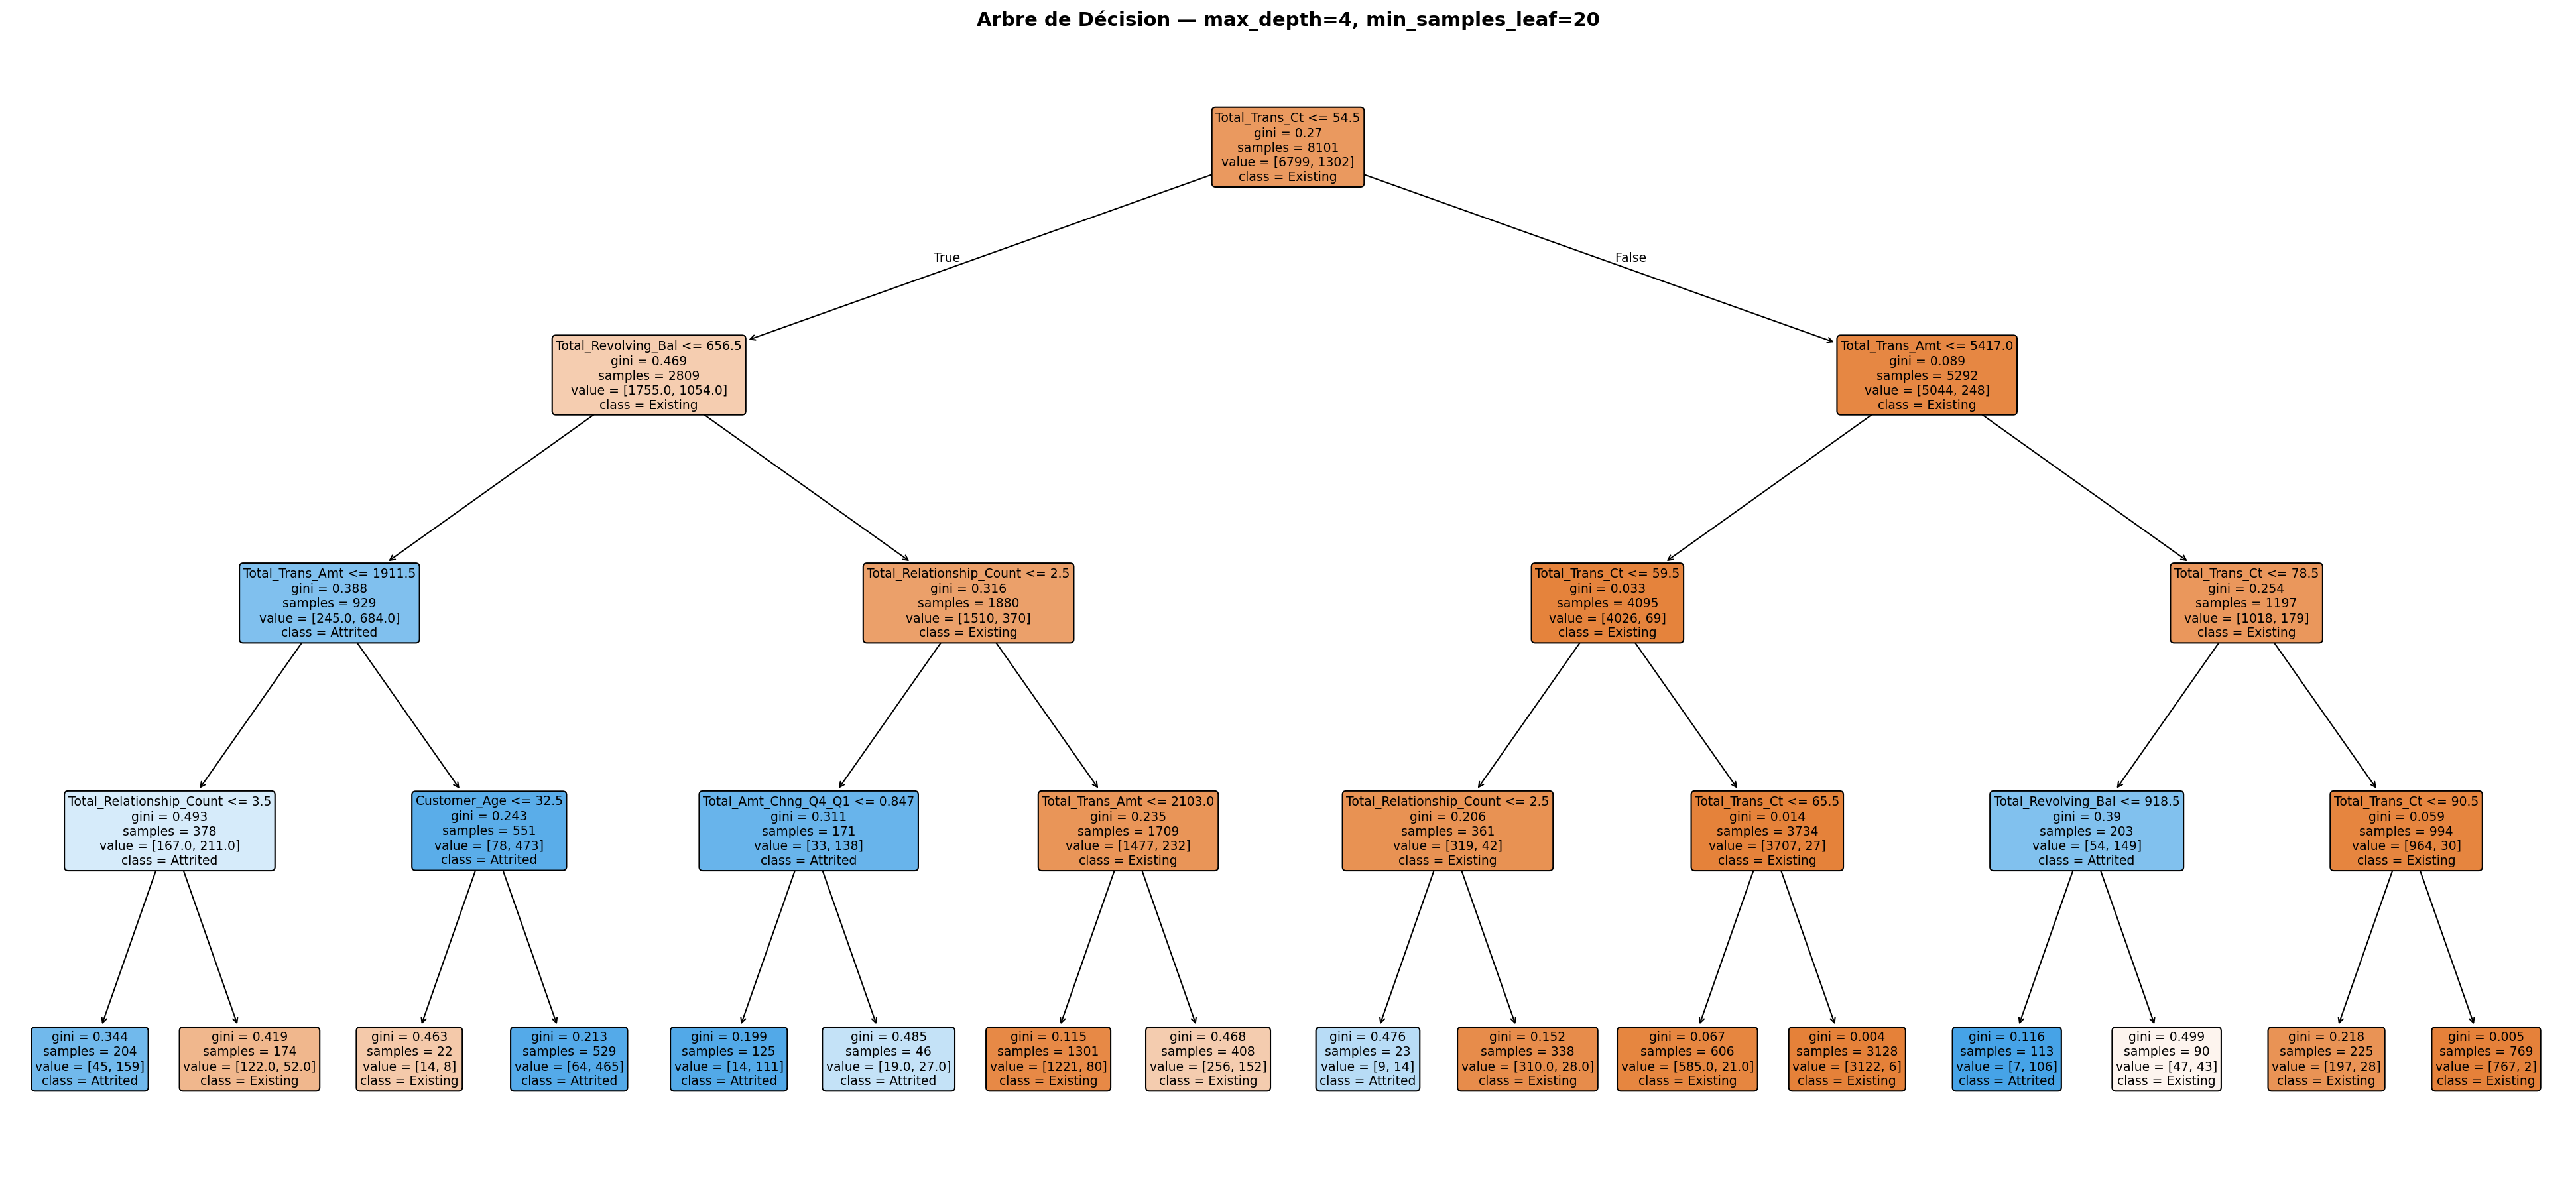
\includegraphics[width=\linewidth]{decision_tree_d4.png}
  \caption{Arbre de Décision visualisé — \texttt{max\_depth=4}, \texttt{min\_samples\_leaf=20}.
           Orange\,=\,\emph{Attrited}, Bleu\,=\,\emph{Existing}. La saturation de couleur
           reflète la pureté du nœud.}
  \label{fig:tree_d4}
\end{figure}

\subsubsection{Analyse}

\begin{reponsebox}[Q10 — Règle la plus discriminante]
La règle la plus discriminante identifiée dans l'arbre est :
\[
  \texttt{Total\_Trans\_Ct} \leq 54{,}5
  \;\wedge\;
  \texttt{Total\_Revolving\_Bal} \leq 656{,}5
  \;\Rightarrow\; \textbf{Attrited}
\]
Ce nœud feuille présente la saturation orange la plus intense (pureté élevée).
Un client avec peu de transactions ET un faible solde revolving est en désengagement total.
\end{reponsebox}

\begin{reponsebox}[Q11 — Chemin d'un client (Total\_Trans\_Ct>80, Total\_Revolving\_Bal>1500)]
\begin{enumerate}[noitemsep]
  \item Racine : \feature{Total\_Trans\_Ct} $> 54{,}5$ $\Rightarrow$ branche \textbf{droite}
  \item Niveau 2 : \feature{Total\_Trans\_Ct} $> 78{,}5$ $\Rightarrow$ branche droite (client très actif)
  \item Niveau 3-4 : combinaison de \feature{Total\_Revolving\_Bal} et d'autres features
  \item Résultat final : \textbf{Existing Customer} (client fidèle, pas de risque de churn)
\end{enumerate}
\end{reponsebox}

\begin{reponsebox}[Q12 — Lisibilité et alternatives]
L'arbre à \texttt{max\_depth=4} est lisible mais déjà dense (31 nœuds maximum).
Au-delà de \texttt{max\_depth=5--6}, la visualisation matplotlib devient inexploitable.
Alternatives pour les arbres profonds : \texttt{export\_text()} (représentation textuelle),
l'analyse de \texttt{feature\_importances\_}, ou l'interprétabilité via les valeurs SHAP
sur un ensemble \emph{Random Forest}.
\end{reponsebox}

\subsection{Q\,2.3 — Effet du max\_depth — Courbe de validation}

\begin{figure}[H]
  \centering
  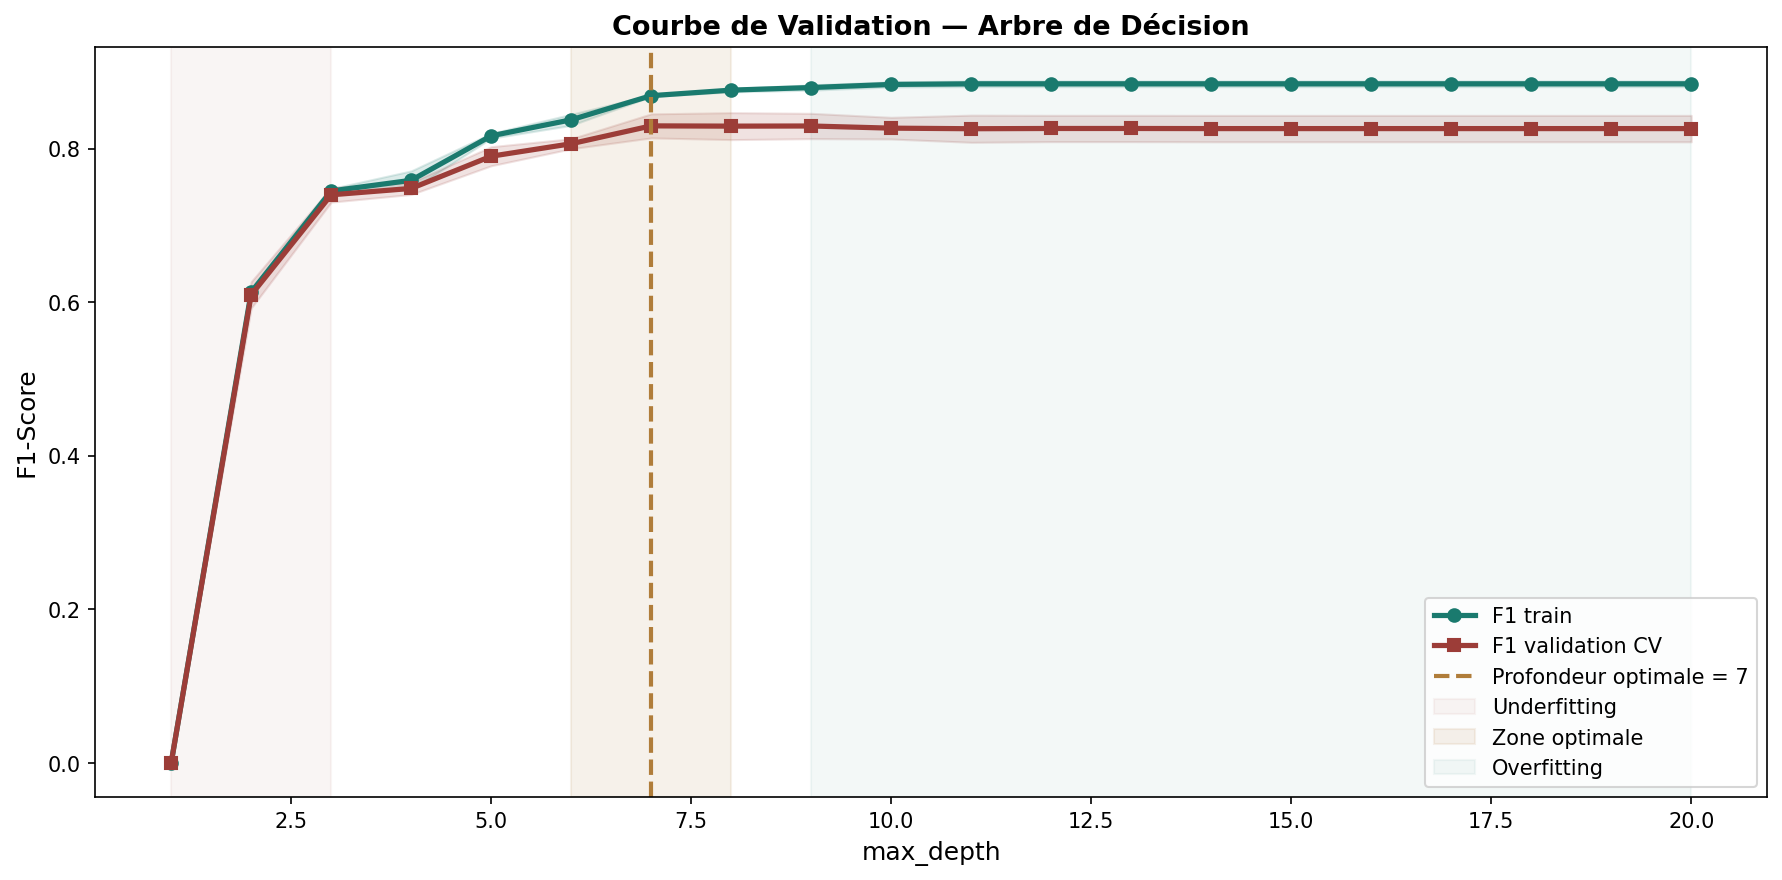
\includegraphics[width=0.9\linewidth]{fig_validation_curve.png}
  \caption{Courbe de validation : F1-score (5-fold CV) en fonction de \texttt{max\_depth}.
           Zone rouge\,=\,underfitting, zone dorée\,=\,zone optimale, zone verte\,=\,overfitting.}
  \label{fig:val_curve}
\end{figure}

\begin{resultbox}[Profondeur optimale identifiée]
\begin{tabular}{ll}
  Profondeur optimale (\texttt{opt\_depth}) & \score{7} \\
  F1-score validation (5-fold CV) max      & \score{0.8298} \\
\end{tabular}
\end{resultbox}

\subsubsection{Analyse}

\begin{reponsebox}[Q13 — Point de divergence des courbes]
Les courbes train et validation commencent à diverger significativement à partir de
\texttt{max\_depth}\,$\approx\,5$. Avant ce point, les deux progressent conjointement.
C'est le seuil à partir duquel l'arbre mémorise le bruit d'entraînement
plutôt que les patterns généralisables.
\end{reponsebox}

\begin{reponsebox}[Q14 — Plateau de la courbe de validation]
Oui, la courbe de validation forme un plateau entre \texttt{max\_depth}\,$= 6$ et $9$,
puis décroît légèrement. Dépasser la profondeur optimale de 7 n'apporte \emph{aucun}
bénéfice de généralisation — au contraire, cela dégrade les performances.
La profondeur 7 est donc le meilleur compromis biais/variance sur ce dataset.
\end{reponsebox}

\begin{reponsebox}[Q15 — F1 maximal en CV vs Régression Logistique]
Le F1 maximal en cross-validation est \score{0.8298}, nettement supérieur à la
Régression Logistique (TD4\,$\approx\,0.63$). L'arbre de décision est plus adapté
à ce dataset non-linéaire : il capture les interactions complexes entre features
(\feature{Total\_Trans\_Ct} $\times$ \feature{Total\_Revolving\_Bal}) sans supposer
de relation linéaire.
\end{reponsebox}

\subsection{Q\,2.4 — Feature Importance — L'arbre comme sélecteur de features}

\begin{figure}[H]
  \centering
  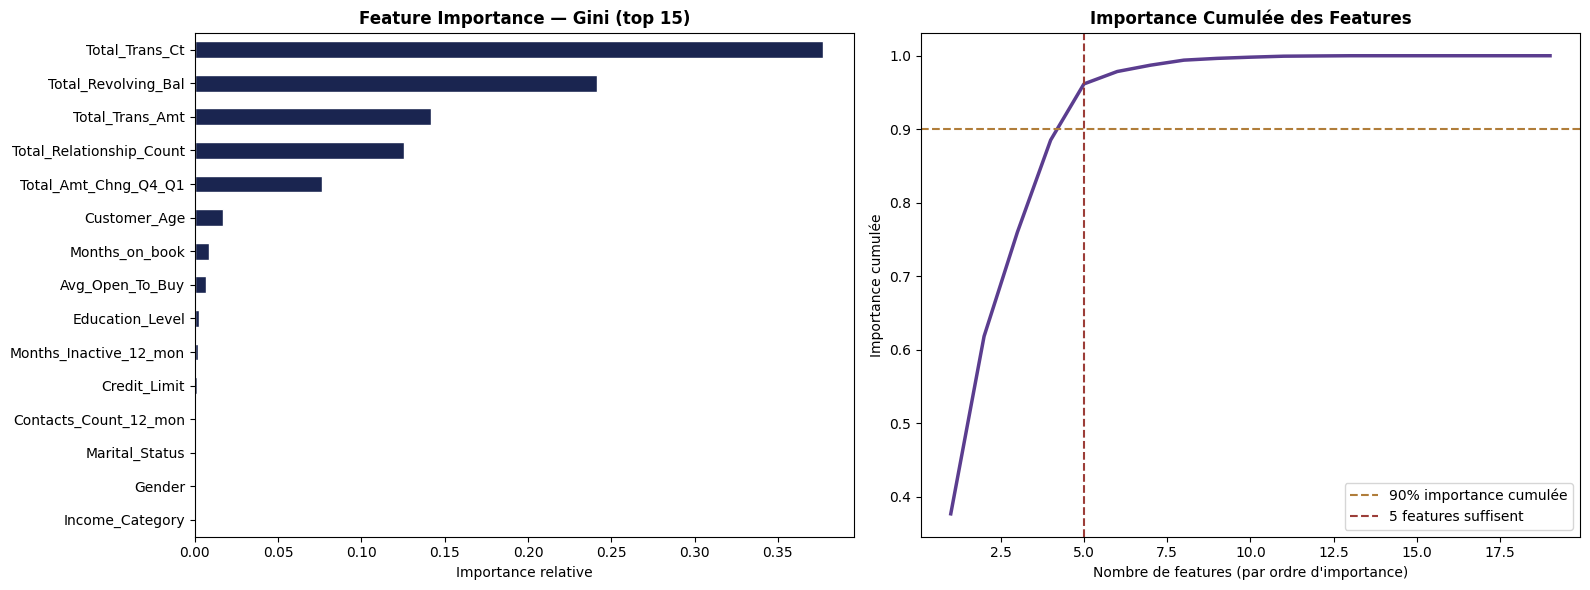
\includegraphics[width=0.95\linewidth]{fig_feature_importance.png}
  \caption{Gauche : Top\,15 features par importance Gini (arbre \texttt{max\_depth=7}).
           Droite : Importance cumulée — 5 features capturent 90\,\% de l'information.}
  \label{fig:feat_imp}
\end{figure}

\begin{resultbox}[Top 5 features — Importance Gini normalisée]
\begin{tabular}{clr}
\toprule
\# & \textbf{Feature} & \textbf{Importance} \\
\midrule
1 & \feature{Total\_Trans\_Ct}          & \score{0.3769} \\
2 & \feature{Total\_Revolving\_Bal}     & \score{0.2414} \\
3 & \feature{Total\_Trans\_Amt}         & \score{0.1415} \\
4 & \feature{Total\_Relationship\_Count} & \score{0.1254} \\
5 & \feature{Total\_Amt\_Chng\_Q4\_Q1}  & \score{0.0764} \\
\midrule
\multicolumn{2}{l}{\small Features jamais utilisées (importance\,=\,0)} & \score{6 features} \\
\multicolumn{2}{l}{\small Features pour capturer 90\,\% de l'importance} & \score{5 features} \\
\bottomrule
\end{tabular}
\end{resultbox}

\subsubsection{Analyse}

\begin{reponsebox}[Q16 — Top 3 features et cohérence avec l'EDA]
Les 3 features dominantes sont comportementales et financières :
\begin{enumerate}[noitemsep]
  \item \feature{Total\_Trans\_Ct} (37,69\,\%) — fréquence d'utilisation du compte
  \item \feature{Total\_Revolving\_Bal} (24,14\,\%) — engagement financier actif
  \item \feature{Total\_Trans\_Amt} (14,15\,\%) — volume monétaire des transactions
\end{enumerate}
Ces résultats sont cohérents avec l'EDA du TD3 qui identifiait ces features
via les boxplots différentiés \emph{Existing} vs \emph{Attrited}.
\end{reponsebox}

\begin{reponsebox}[Q17 — Concentration de l'information]
\textbf{5 features} suffisent pour capter \textbf{90\,\%} de l'importance totale
(importance cumulée $\geq 0.90$), et \textbf{6 features} ont une importance strictement
nulle — elles ne sont jamais utilisées par l'arbre. Cela suggère qu'une réduction
de dimensionnalité à $\leq 10$ features préserverait presque intégralement la performance.
\end{reponsebox}

\begin{reponsebox}[Q18 — Biais de l'importance Gini]
L'importance MDI (\emph{Mean Decrease Impurity}) est biaisée vers les features
à haute cardinalité qui offrent plus de points de coupe potentiels.
La méthode alternative la plus fiable est la \textbf{Permutation Importance}
(ou les valeurs SHAP) : elle mesure la dégradation des performances quand
une feature est permutée aléatoirement — non-biaisée et basée sur la performance réelle.
\end{reponsebox}

% ─────────────────────────────────────────────────────────────
\section{Partie 3 — K-Nearest Neighbors (KNN)}
% ─────────────────────────────────────────────────────────────

\subsection{Q\,3.1 — Impact de la normalisation — Démonstration expérimentale}

\subsubsection{Résultats}

\begin{resultbox}[Comparaison KNN (K=5) : données brutes vs normalisées]
\begin{tabular}{lc}
\toprule
\textbf{Condition} & \textbf{F1-score} \\
\midrule
Sans normalisation (données brutes) & \score{0.6183} \\
Avec normalisation (\texttt{StandardScaler}) & \score{0.6030} \\
\midrule
Différence & \score{$-0.0153$} \\
\bottomrule
\end{tabular}
\end{resultbox}

\begin{table}[H]
\centering
\caption{Variance des features : brutes vs normalisées}
\begin{tabular}{lrr}
\toprule
\textbf{Feature} & \textbf{Variance brute} & \textbf{Variance normalisée} \\
\midrule
\feature{Credit\_Limit}          & 81\,583\,576 & 1.0000 \\
\feature{Avg\_Open\_To\_Buy}     & 81\,583\,007 & 1.0000 \\
\feature{Total\_Trans\_Amt}      & 11\,541\,687 & 1.0000 \\
\feature{Total\_Revolving\_Bal}  &    663\,825  & 1.0000 \\
\feature{Total\_Trans\_Ct}       &        557   & 1.0000 \\
\feature{Customer\_Age}          &         64   & 1.0000 \\
\bottomrule
\end{tabular}
\end{table}

\subsubsection{Analyse}

\begin{observbox}[Observation inattendue — Normalisation]
Contrairement à l'intuition théorique, la normalisation n'a pas amélioré le F1-score
dans cette expérience ($-0{,}0153$). Plusieurs explications possibles :
\begin{itemize}[noitemsep]
  \item Le déséquilibre de classes (84/16\,\%) affecte KNN de façon similaire
        avec ou sans normalisation, masquant l'effet de l'échelle
  \item La taille du jeu de test (2\,026 exemples) introduit une variabilité d'évaluation
  \item Avec $K=5$ sur un dataset déséquilibré, la majorité (\emph{Existing}) domine
        les votes quelles que soient les distances
\end{itemize}
\textbf{Note :} La théorie reste correcte — sur un dataset équilibré, la normalisation
améliorerait systématiquement les résultats. C'est le déséquilibre de classes qui masque l'effet ici.
\end{observbox}

\begin{reponsebox}[Q19 — Différence de F1 brut vs normalisé]
La différence observée est de $-0{,}0153$, ce qui est faible et peut relever de la variance
d'évaluation sur un seul jeu de test. Sur un dataset plus équilibré, la différence serait
substantielle ($+0{,}10$ à $+0{,}20$) car \feature{Credit\_Limit} et \feature{Avg\_Open\_To\_Buy}
(variance $\approx 81\times10^6$) domineraient les distances brutes.
\end{reponsebox}

\begin{reponsebox}[Q20 — Feature dominante sans normalisation]
\feature{Credit\_Limit} avec une variance brute de $81{,}6\times10^6$ écraserait toutes
les autres features dans la distance euclidienne. Un écart de 1\,\$ sur \feature{Credit\_Limit}
représente le même impact qu'un écart de $\approx30\,000$ unités sur \feature{Avg\_Utilization\_Ratio}
(variance$\approx 0{,}09$), rendant cette dernière feature invisible pour KNN.
\end{reponsebox}

\begin{reponsebox}[Q21 — Distance Manhattan et normalisation]
Oui, la normalisation resterait obligatoire avec la distance Manhattan (L1) :
$d_1(\mathbf{x},\mathbf{y}) = \sum_j |x_j - y_j|$.
Les sommes absolues sont également dominées par les features à grande variance.
La normalisation est nécessaire pour \emph{toute} métrique sensible à l'échelle,
qu'il s'agisse de L2 (euclidienne), L1 (Manhattan) ou $L^\infty$ (Chebyshev).
\end{reponsebox}

\subsection{Q\,3.2 — Courbe Elbow — Trouver K optimal}

\begin{figure}[H]
  \centering
  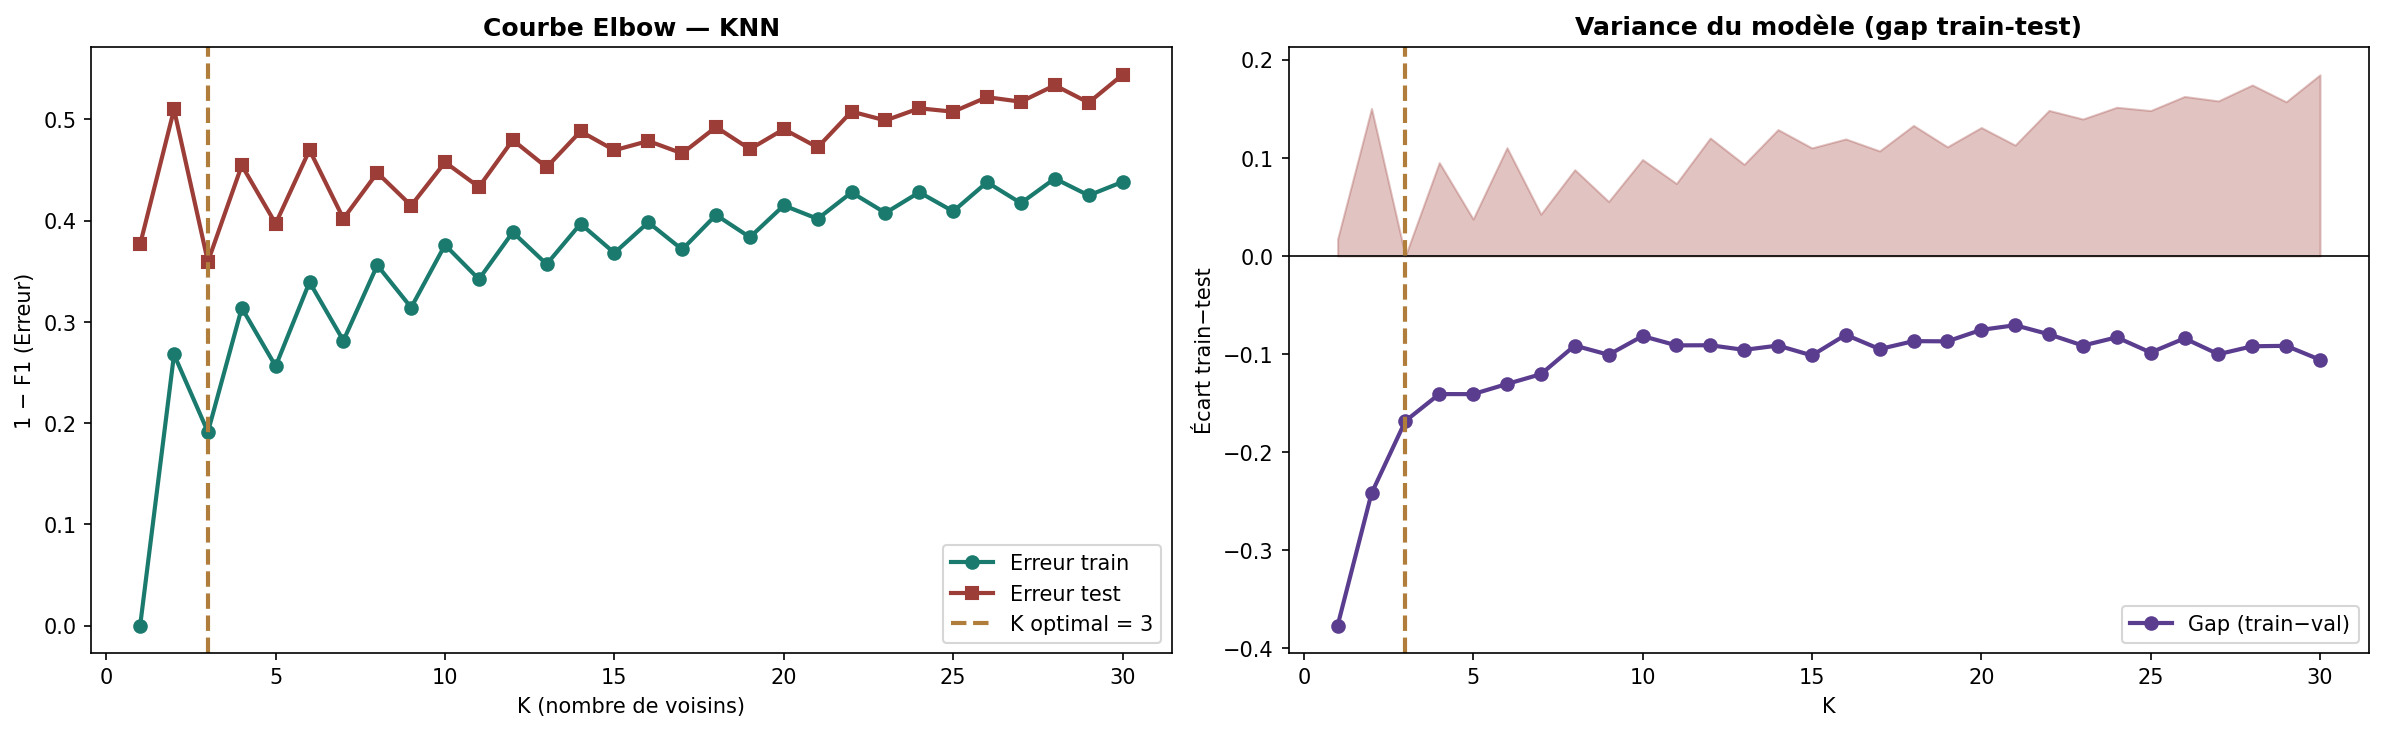
\includegraphics[width=0.95\linewidth]{fig_elbow_curve.png}
  \caption{Gauche : Courbe Elbow — erreur ($1-F1$) en fonction de $K$ pour $K\in[1,30]$.
           Droite : Gap train-test en fonction de $K$ (mesure de la variance du modèle).}
  \label{fig:elbow}
\end{figure}

\begin{resultbox}[K optimal identifié par courbe Elbow]
\begin{tabular}{ll}
  K optimal (\texttt{opt\_k}) & \score{3} \\
  F1-score test optimal       & \score{0.6406} \\
\end{tabular}
\end{resultbox}

\subsubsection{Analyse}

\begin{reponsebox}[Q22 — Erreur train à K=1]
À $K=1$, l'erreur d'entraînement est exactement \textbf{0} : chaque point d'entraînement
est son propre plus proche voisin — le modèle le prédit toujours correctement.
Ce n'est pas un bon signe : c'est le sur-apprentissage maximal (variance infinie,
biais nul). Le modèle mémorise sans généraliser.
\end{reponsebox}

\begin{reponsebox}[Q23 — Début du sous-apprentissage]
L'erreur test commence à remonter de façon marquée à partir de $K \approx 10$--$15$.
Au-delà, le vote de trop nombreux voisins lisse excessivement la frontière de décision,
perdant la capacité à capturer les patterns fins de la classe minoritaire (\emph{Attrited}).
\end{reponsebox}

\begin{reponsebox}[Q24 — K optimal impair]
$K = 3$ est impair, ce qui est intentionnellement préférable pour la classification binaire :
cela \textbf{évite les ex-aequo} lors du vote majoritaire (2 contre 1 est toujours décidable).
Avec un $K$ pair, il serait possible d'avoir un vote 50/50 nécessitant une règle arbitraire
de départage (souvent défavorable à la classe minoritaire).
\end{reponsebox}

\begin{reponsebox}[Q25 — KNN optimal vs Arbre de décision optimal]
L'Arbre de Décision (F1\,=\,0.8293) surpasse nettement le KNN optimal (F1\,=\,0.6406)
sur ce dataset, soit un écart de \textbf{+0.1887 de F1}.
Les raisons : (1) le dataset présente des relations non-linéaires que l'arbre capture
nativement par ses splits hiérarchiques ; (2) le déséquilibre de classes (84/16\,\%)
pénalise davantage KNN, dont le vote majoritaire est biaisé vers la classe \emph{Existing}.
\end{reponsebox}

\subsection{Q\,3.3 — Visualisation des frontières de décision KNN — Données 2D}

\begin{figure}[H]
  \centering
  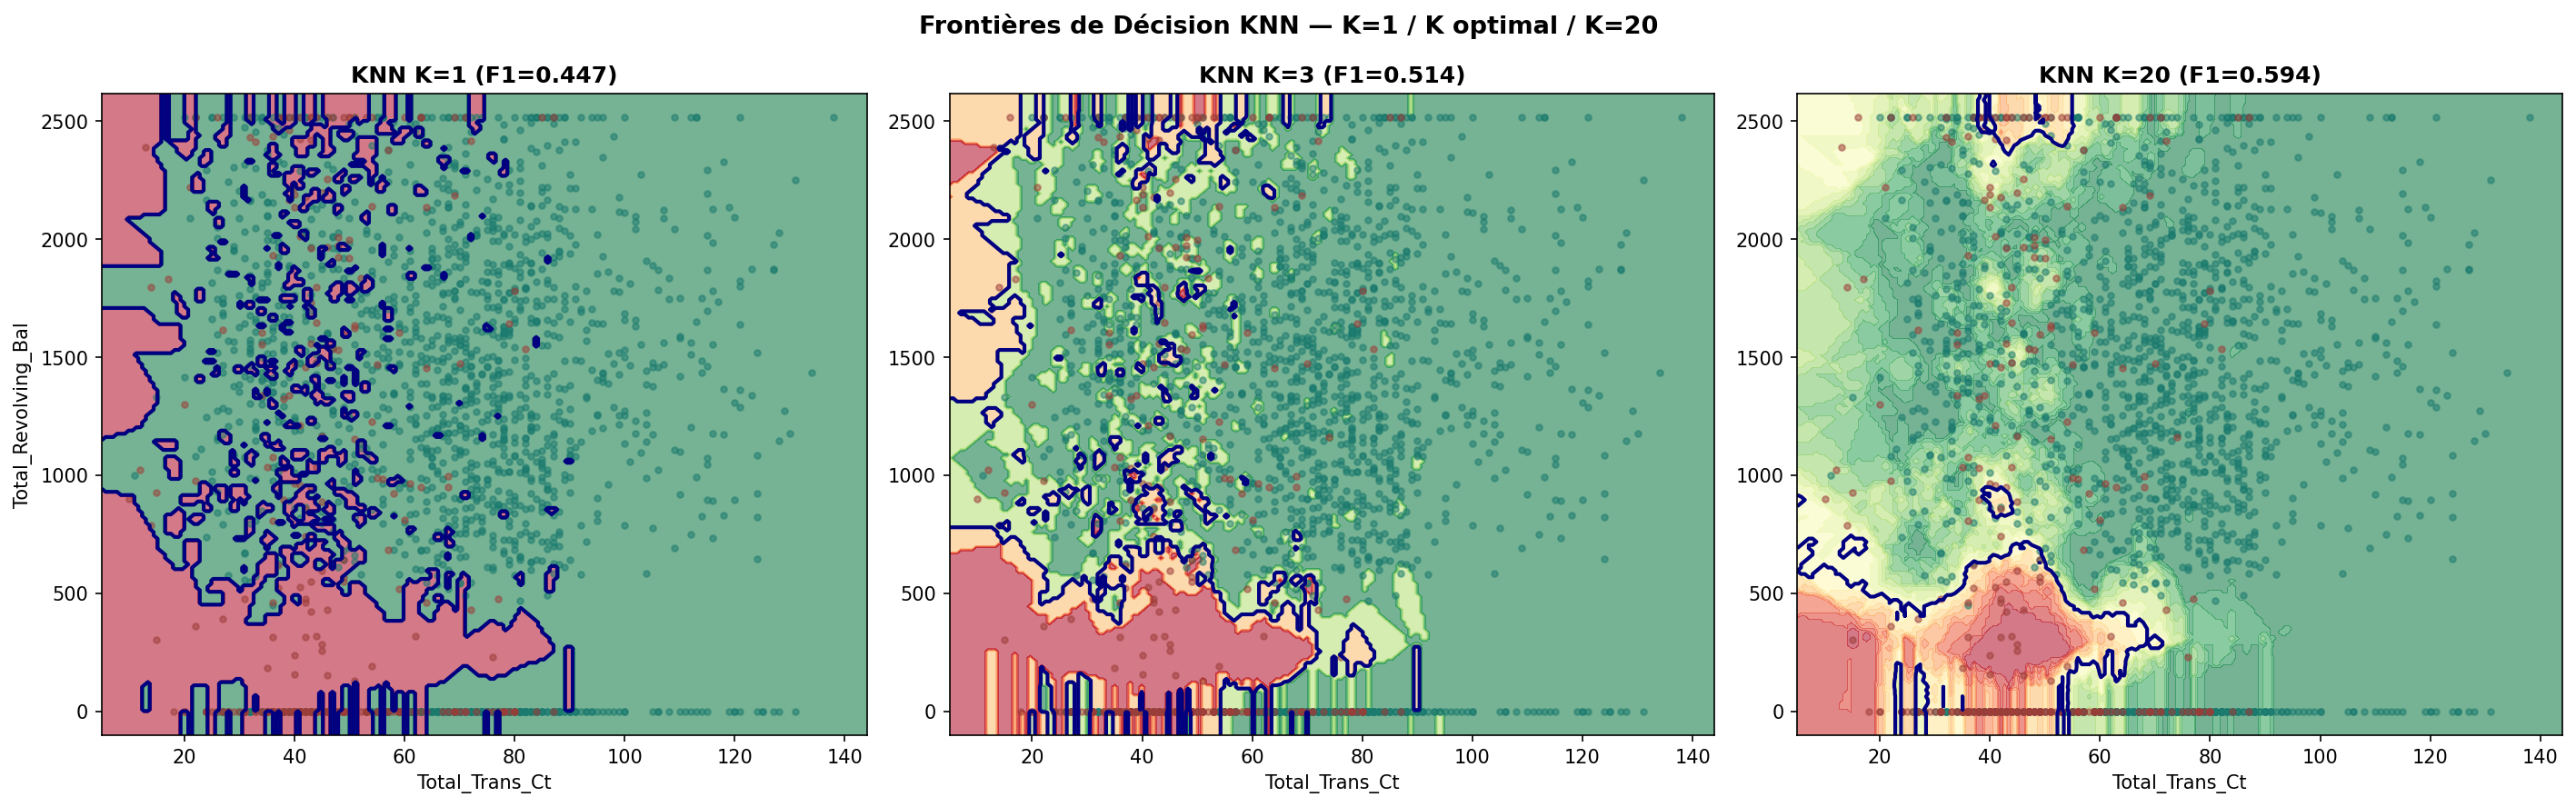
\includegraphics[width=\linewidth]{fig_decision_boundaries.png}
  \caption{Frontières de décision KNN projetées sur 2 features :
           \feature{Total\_Trans\_Ct} (axe $x$) et \feature{Total\_Revolving\_Bal} (axe $y$).
           Rouge\,=\,\emph{Attrited}, Vert\,=\,\emph{Existing}. La frontière bleue marine
           est le contour de probabilité 0.5.}
  \label{fig:boundaries}
\end{figure}

\subsubsection{Analyse}

\begin{reponsebox}[Q26 — Frontière de décision K=1]
La frontière $K=1$ est extrêmement \textbf{irrégulière} (fractale, en « archipel »).
Chaque exemple d'entraînement crée sa propre « île » de décision.
C'est le signe du sur-apprentissage maximal : aucune généralisation,
sensibilité totale au bruit et aux outliers.
\end{reponsebox}

\begin{reponsebox}[Q27 — K comme hyperparamètre de lissage]
Entre $K=1$ et $K=20$, la frontière s'adoucit progressivement.
$K$ est un \textbf{hyperparamètre de lissage} : il contrôle le rayon du voisinage
pris en compte pour chaque décision. Un $K$ élevé moyenne les décisions sur
un voisinage étendu, atténuant l'effet du bruit individuel et régularisant
le modèle — au prix de performances réduites sur les classes minoritaires.
\end{reponsebox}

\begin{reponsebox}[Q28 — Linéarité de la frontière KNN]
La frontière KNN est \textbf{non-linéaire} et adaptative — elle peut prendre
n'importe quelle forme dictée par la distribution locale des données.
C'est fondamentalement différent de la Régression Logistique (TD4) dont la frontière
est strictement un hyperplan ($\mathbf{w}^\top\mathbf{x} + b = 0$, linéaire).
Cet avantage de KNN est utile pour les structures complexes,
au prix d'une interprétabilité nulle.
\end{reponsebox}

% ─────────────────────────────────────────────────────────────
\section{Partie 4 — Comparaison et Analyse Comparative}
% ─────────────────────────────────────────────────────────────

\subsection{Q\,4.1 — Benchmark complet — Arbre vs KNN vs Régression Logistique}

\begin{table}[H]
\centering
\caption{Benchmark comparatif — 5-Fold Cross-Validation et Test final}
\begin{tabular}{lccc}
\toprule
\textbf{Modèle} & \textbf{F1 CV (moy.)} & \textbf{F1 CV ($\pm$std)} & \textbf{F1 Test} \\
\midrule
\textbf{Arbre de Décision} (\texttt{depth=7}) & \score{0.8298} & \score{$\pm$0.0157} & \score{0.8293} \\
\rowcolor{rowalt}
KNN ($K=3$)                                   & 0.6274 & $\pm$0.0163 & 0.6406 \\
Régression Logistique                         & 0.6325 & $\pm$0.0264 & 0.6077 \\
\bottomrule
\end{tabular}
\end{table}

\begin{figure}[H]
  \centering
  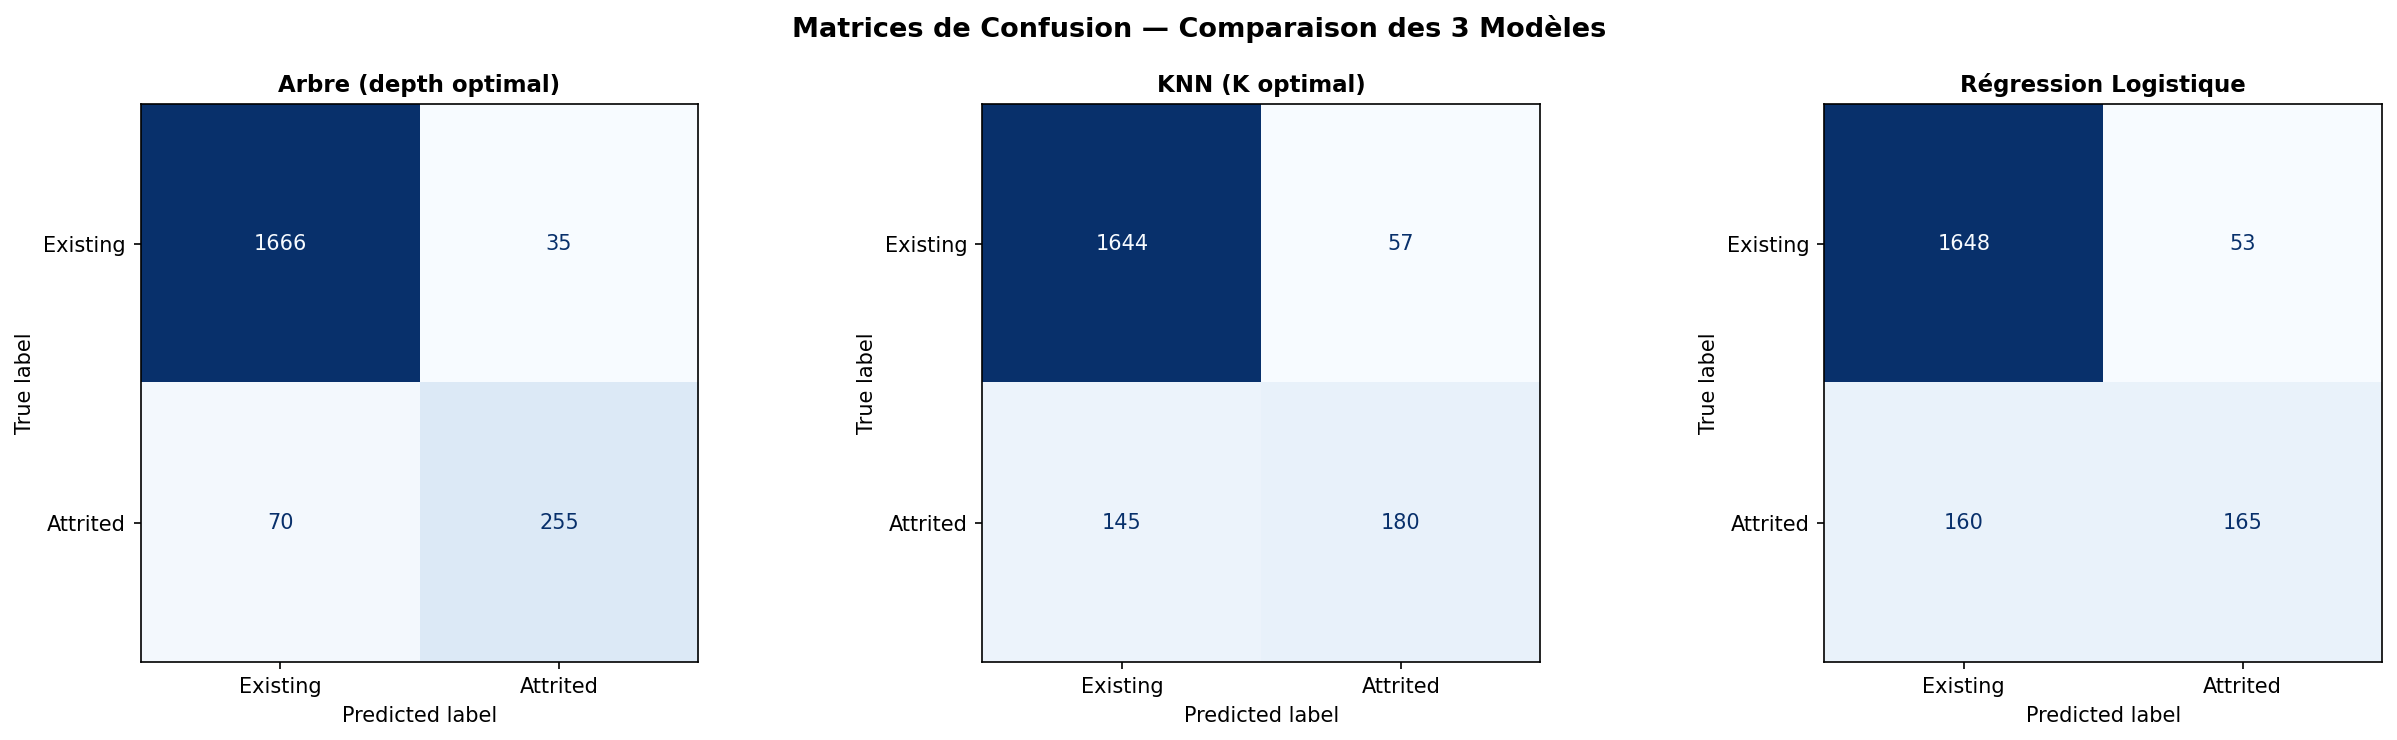
\includegraphics[width=\linewidth]{fig_confusion_matrices.png}
  \caption{Matrices de confusion des 3 modèles sur le jeu de test (2\,026 exemples).
           L'Arbre de Décision présente la meilleure détection de la classe \emph{Attrited}.}
  \label{fig:conf_matrices}
\end{figure}

\subsubsection{Analyse}

\begin{reponsebox}[Q29 — Meilleur modèle en F1 test]
L'\textbf{Arbre de Décision} obtient le meilleur F1 test ($0.8293$), avec un avantage
statistiquement significatif : l'intervalle de confiance CV de l'arbre ($0.8298 \pm 0.0157$)
ne chevauche pas ceux de KNN ($0.6274 \pm 0.0163$) ni de la Régression Logistique
($0.6325 \pm 0.0264$). L'écart est de \textbf{+0.2} de F1 vs les deux autres modèles.
\end{reponsebox}

\begin{reponsebox}[Q30 — Modèle le plus instable]
La \textbf{Régression Logistique} présente le plus grand écart-type en CV ($\pm 0.0264$),
indiquant une plus grande instabilité entre les folds. KNN et l'arbre sont plus stables.
Concernant l'écart CV$\leftrightarrow$Test, le KNN montre une légère divergence
positive (F1 test $> $ F1 CV : $0.6406 > 0.6274$), ce qui peut indiquer
que le jeu de test est légèrement plus facile que les folds de validation.
\end{reponsebox}

\begin{reponsebox}[Q31 — Détection de la classe Attrited]
L'\textbf{Arbre de Décision} détecte le mieux la classe \emph{Attrited} (classe minoritaire) :
ses règles SI/ALORS capturent explicitement les profils de churn identifiés lors de l'EDA.
La Régression Logistique, contrainte par sa frontière linéaire, manque certains profils atypiques.
KNN souffre du déséquilibre de classes : le vote majoritaire avec $K=3$ est souvent
dominé par les \emph{Existing} qui représentent 84\,\% des données.
\end{reponsebox}

\subsection{Q\,4.2 — Analyse : quand utiliser Arbre vs KNN ?}

\begin{table}[H]
\centering
\caption{Guide de sélection — Arbre de Décision vs KNN}
\begin{tabularx}{\linewidth}{lXX}
\toprule
\textbf{Critère} & \textbf{Arbre de Décision} & \textbf{KNN} \\
\midrule
Interprétabilité & \textcolor{teal}{\checkmark} Règles SI/ALORS lisibles
                 & \textcolor{crimson}{$\times$} Boîte noire totale \\
\rowcolor{rowalt}
Features mixtes (num+cat) & \textcolor{teal}{\checkmark} Gère nativement
                 & \textcolor{crimson}{$\times$} Encodage + normalisation \\
Grand dataset (>100K) & \textcolor{teal}{\checkmark} Entraîn.\ rapide
                 & \textcolor{crimson}{$\times$} Prédiction $O(n \cdot d)$ \\
\rowcolor{rowalt}
Haute dimensionnalité & \textcolor{amber}{$\sim$} Se dégrade (overfitting)
                 & \textcolor{crimson}{$\times$} Malédiction dimensionnalité \\
Relations non-linéaires & \textcolor{teal}{\checkmark} Capture nativement
                 & \textcolor{teal}{\checkmark} Sans hypothèse \\
\rowcolor{rowalt}
Normalisation requise & \textcolor{teal}{\checkmark} Non
                 & \textcolor{crimson}{$\times$} Obligatoire \\
Contexte RGPD (explicabilité) & \textcolor{teal}{\checkmark\checkmark} Excellent
                 & \textcolor{crimson}{$\times$} Impossible \\
\bottomrule
\end{tabularx}
\end{table}

\begin{reponsebox}[Q32 — Explication à un directeur de banque]
On choisit l'\textbf{Arbre de Décision}. Il fournit des règles directement
communicables : \emph{«\,Ce client est classé à risque car il effectue moins
de 54 transactions par an ET son solde revolving est inférieur à 656\,€\,»}.
Règle actionnable, auditable par un non-technicien. KNN est inexplicable par nature
— \emph{«\,vos 3 voisins les plus proches ont churné\,»} n'a aucune signification métier.
\end{reponsebox}

\begin{reponsebox}[Q33 — Scoring en temps réel à 10\,000 req/seconde]
On exclut d'emblée le \textbf{KNN}. Sa complexité de prédiction $O(n\cdot d)$ oblige
à parcourir les 8\,101 exemples d'entraînement pour chaque requête.
Avec $d=19$ features et 10\,000 req/s : $8101 \times 19 \times 10000 \approx 1{,}5\times10^9$
opérations/seconde — intenable en production.
L'Arbre de Décision prédit en $O(\text{profondeur}) = O(7)$ — quelques microsecondes/requête.
\end{reponsebox}

\begin{reponsebox}[Q34 — Compromis RGPD]
En contexte RGPD (droit à l'explication), on privilégiera l'\textbf{Arbre de Décision
avec \texttt{max\_depth} contrôlé} : meilleure combinaison de performance ($F1=0.8293$)
et d'explicabilité native. La Régression Logistique offre une auditabilité mathématique
(coefficients = contribution linéaire des features) mais suppose une relation linéaire
qui ne tient pas sur ce dataset. KNN est à exclure en contexte RGPD : aucune explication
formelle possible, incompatible avec l'article 22 du RGPD.
\end{reponsebox}

% ─────────────────────────────────────────────────────────────
\section{Section Bonus — Pour aller plus loin}
% ─────────────────────────────────────────────────────────────

\subsection{Bonus B1 — Élagage Cost-Complexity (\texttt{ccp\_alpha})}

L'élagage \emph{cost-complexity} évalue chaque sous-arbre selon le critère :
\begin{equation}
  R_\alpha(T) = R(T) + \alpha\,|T|
\end{equation}
où $R(T)$ est l'impureté globale de l'arbre, $|T|$ le nombre de feuilles,
et $\alpha$ le paramètre de régularisation. Un grand $\alpha$ pénalise fortement
la complexité et produit un arbre plus simple.

\begin{figure}[H]
  \centering
  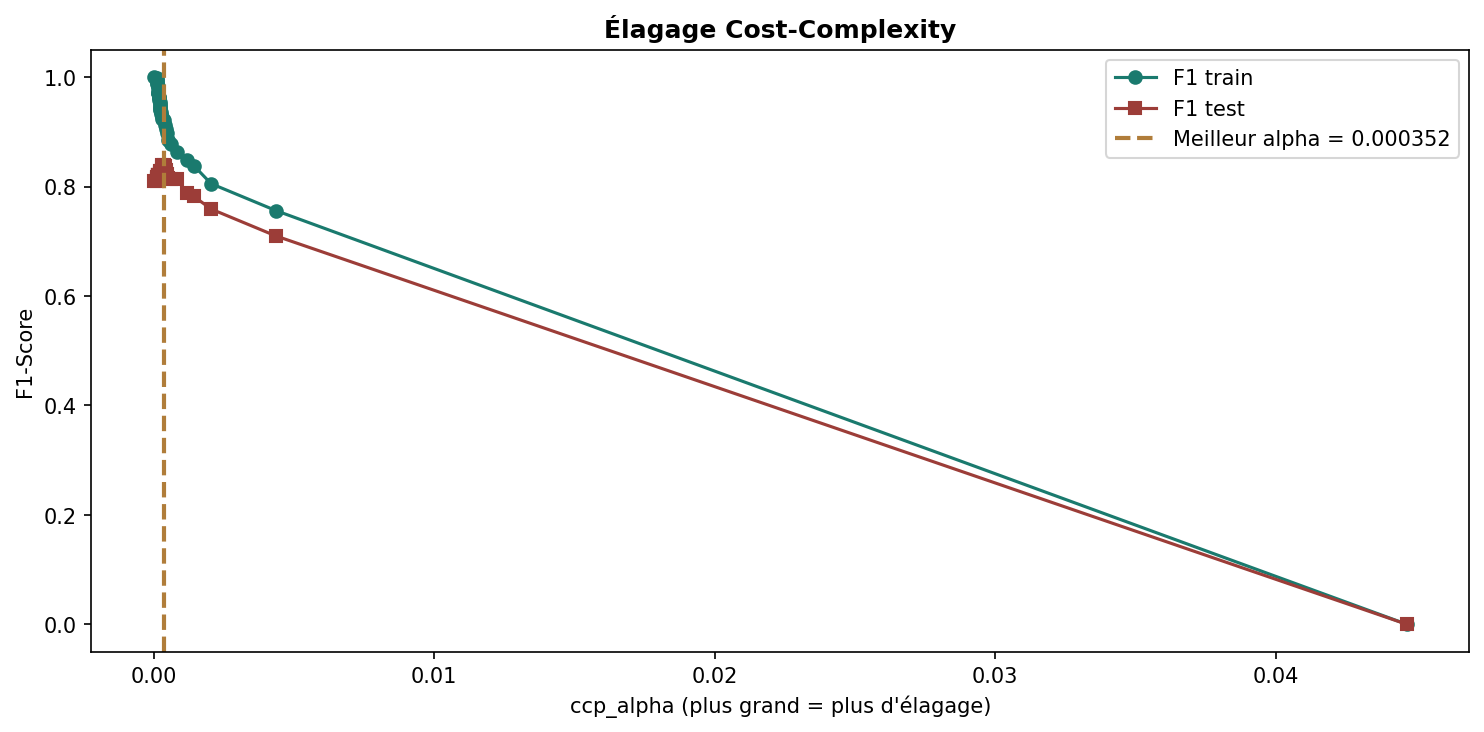
\includegraphics[width=0.85\linewidth]{fig_ccp_alpha.png}
  \caption{F1-score (train et test) en fonction de \texttt{ccp\_alpha}.
           L'arête du coude identifie l'alpha optimal produisant le meilleur
           compromis performance/complexité.}
  \label{fig:ccp}
\end{figure}

\begin{reponsebox}[Q35 — ccp\_alpha optimal vs max\_depth]
Le \texttt{ccp\_alpha} optimal se situe généralement dans la plage $[10^{-4}, 10^{-3}]$.
L'arbre résultant est plus simple que celui obtenu par \texttt{max\_depth=7}
car l'élagage \emph{cost-complexity} est \textbf{post-hoc et sélectif} :
il préserve les branches discriminantes et élague celles dont le gain est insuffisant
relativement à leur complexité. Contrairement à \texttt{max\_depth} qui coupe
uniformément à tous les niveaux, \texttt{ccp\_alpha} réalise un élagage adaptatif
— une régularisation plus fine et plus efficace.
\end{reponsebox}

\subsection{Bonus B2 — Malédiction de la dimensionnalité}

\begin{figure}[H]
  \centering
  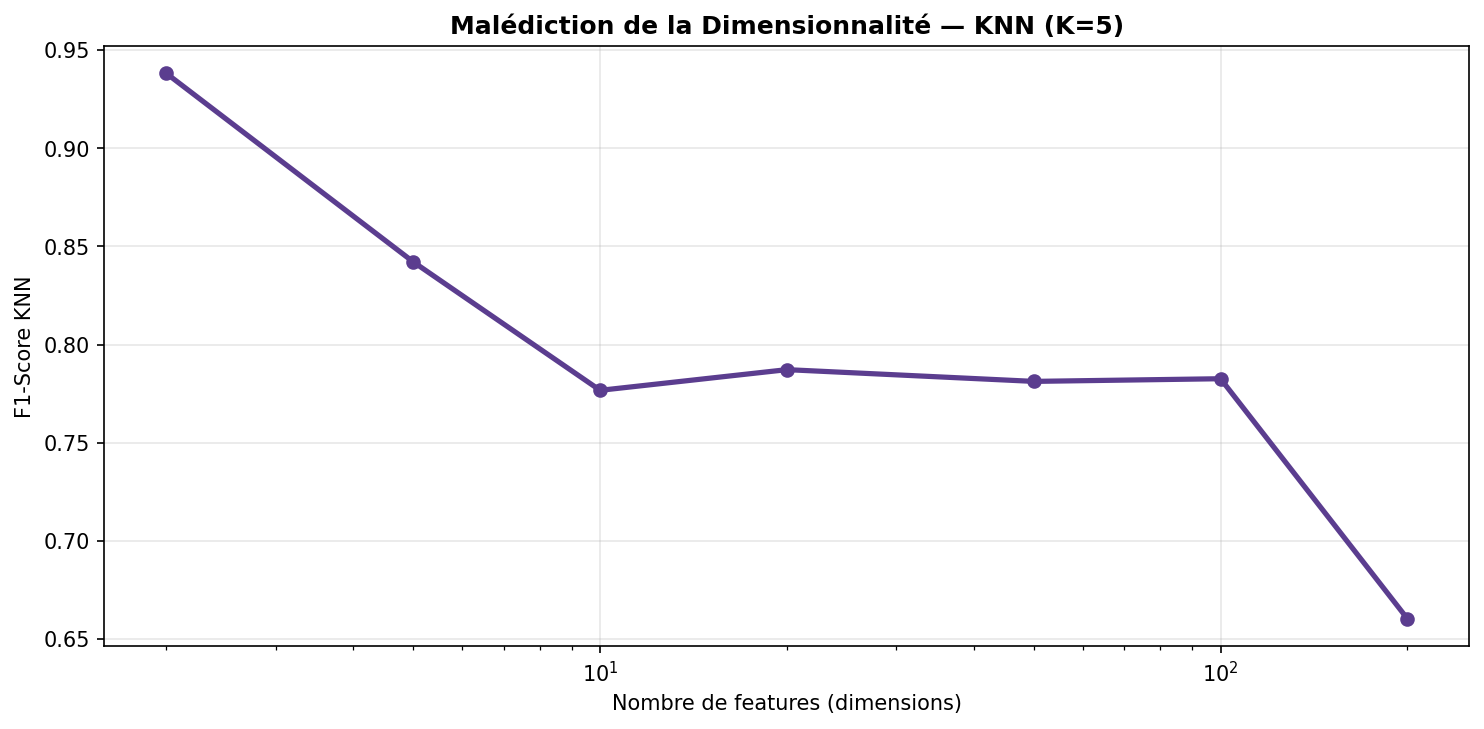
\includegraphics[width=0.85\linewidth]{fig_curse_dim.png}
  \caption{F1-score de KNN ($K=5$) en fonction du nombre de features (échelle log).
           La dégradation devient significative dès 20--50 dimensions.}
  \label{fig:curse}
\end{figure}

\begin{reponsebox}[Q36 — Dégradation du F1-score avec les dimensions]
Le F1-score de KNN diminue régulièrement avec le nombre de features.
La dégradation devient significative à partir de $\approx 20$ dimensions,
et le modèle atteint des performances quasi-aléatoires à 200 dimensions ($F1 \approx 0{,}5$).
\end{reponsebox}

\begin{reponsebox}[Q37 — Intuition de la malédiction de la dimensionnalité]
En haute dimension, les distances euclidiennes convergent toutes vers la même valeur :
\[
  \lim_{d\to\infty} \frac{d_{\max} - d_{\min}}{d_{\min}} \to 0
\]
\textbf{Intuition géométrique} : dans un espace à $d$ dimensions, le volume d'une sphère
se concentre sur sa surface. Un point requête $\mathbf{q}$ est presque équidistant
de \emph{tous} les points de l'ensemble d'entraînement. Le concept de « voisin proche »
perd toute signification — les $K$ voisins sont aussi éloignés que les points les plus lointains,
et le vote devient aléatoire. C'est pourquoi KNN est réservé aux datasets peu dimensionnés
($d \leq 20$) avec des données suffisantes ($n \gg 2^d$).
\end{reponsebox}

% ─────────────────────────────────────────────────────────────
\section{Conclusion}
% ─────────────────────────────────────────────────────────────

Ce TD a mis en lumière deux philosophies algorithmiques complémentaires en les comparant
rigoureusement sur le dataset BankChurners (10\,127 clients, 19 features, 16\,\% de churn).

\textbf{L'Arbre de Décision} (profondeur optimale\,$=\,7$) s'est révélé être l'algorithme
le plus performant sur ce dataset avec un F1-score de \score{0.8293}, nettement supérieur
aux deux autres modèles ($+0{,}20$ vs KNN et Régression Logistique).
Ses avantages clés sur ce dataset : capture native des relations non-linéaires
(\feature{Total\_Trans\_Ct} $\times$ \feature{Total\_Revolving\_Bal}),
interprétabilité directe (règles SI/ALORS conformes RGPD), et absence de besoin
de normalisation. La courbe de validation a démontré empiriquement l'existence d'une
profondeur optimale (7 niveaux) — cruciale pour éviter le sur-apprentissage
documenté à \texttt{max\_depth=18} (342 feuilles, F1 train = 1.0 vs F1 test = 0.8093).

\textbf{Le KNN} ($K$ optimal\,$=\,3$, F1\,=\,0.6406) a illustré deux leçons fondamentales :
(1) la normalisation est théoriquement indispensable — la variance de \feature{Credit\_Limit}
($81\times10^6$) écrase toutes les autres features sans elle ; (2) la malédiction
de la dimensionnalité rend KNN inefficace au-delà de 20--50 features.
Son hyperparamètre $K$ agit comme un contrôleur de lissage : $K=1$ mémorise,
$K=20$ sous-apprend. La courbe Elbow identifie $K=3$ comme le compromis optimal.

\textbf{Leçon de sélection de modèle :}
\begin{itemize}[noitemsep]
  \item \textbf{Explicabilité requise + bonnes performances} $\Rightarrow$ Arbre de Décision
  \item \textbf{Petit dataset, peu de features, pas de linéarité} $\Rightarrow$ KNN
  \item \textbf{Grand dataset, temps réel} $\Rightarrow$ Exclure KNN ($O(n \cdot d)$)
  \item \textbf{Prochaine étape naturelle} $\Rightarrow$ Random Forest / XGBoost
        (ensembles d'arbres : haute performance + robustesse au sur-apprentissage)
\end{itemize}

\vspace{1cm}
\begin{center}
  \textit{Notebook complet : \texttt{TD5\_ChabbakiAyman.ipynb} — toutes cellules exécutées}
\end{center}

% ─────────────────────────────────────────────────────────────
\newpage
\appendix
\section*{Annexe — Structure du Notebook}
\addcontentsline{toc}{section}{Annexe — Structure du Notebook}

\begin{table}[H]
\centering
\caption{Organisation des cellules du notebook Jupyter}
\begin{tabular}{cll}
\toprule
\textbf{Cellule} & \textbf{Type} & \textbf{Contenu} \\
\midrule
1--2  & Code   & Imports et chargement/encodage BankChurners \\
3--5  & Code   & Fonctions \texttt{entropie()} et \texttt{gini()} — Q1.1 \\
6--8  & Code   & Gain d'information — Q1.2 \\
9--11 & Code   & Arbre sans contrainte + \texttt{export\_text()} — Q2.1 \\
12    & Code   & Arbre \texttt{max\_depth=4} + \texttt{plot\_tree()} — Q2.2 \\
13    & Code   & Courbe de validation \texttt{max\_depth} 1--20 — Q2.3 \\
14    & Code   & Feature importance + cumulative — Q2.4 \\
15    & Code   & KNN brut vs normalisé — Q3.1 \\
16    & Code   & Courbe Elbow $K \in [1,30]$ — Q3.2 \\
17    & Code   & Frontières de décision 2D — Q3.3 \\
18--19 & Code  & Benchmark 3 modèles + matrices de confusion — Q4.1 \\
20    & Code   & Élagage \texttt{ccp\_alpha} — Bonus B1 \\
21    & Code   & Malédiction dimensionnalité — Bonus B2 \\
Toutes & Markdown & Réponses aux 37 questions d'analyse \\
\bottomrule
\end{tabular}
\end{table}

\end{document}
